%Preambolo per documento generico
%Per cambiare tipo di documento modificare
%il documentclass.

\documentclass[11pt]{article}
\usepackage[utf8]{inputenc}

%Mettere italian se si vuole scrivere in italiano
\usepackage[english]{babel}


%Aumento dell'interlinea
\usepackage{setspace}
\onehalfspacing

%Pacchetti per simboli matematici
\usepackage{mathtools}
\usepackage{amsfonts}
\usepackage{amsthm}
\newtheorem{theorem}{Theorem}
\usepackage{amsmath}
\usepackage{bm}


%Pacchetti per figure e tabelle
\usepackage{booktabs, caption, graphicx, subfig, float}
\captionsetup{tableposition=top,figureposition=bottom,font=small}

%Per inserire commenti in blocco
%Usage: \begin{comment} ... \end{comment}
\usepackage{comment}

%Definisce colori dei link nel testo e altri parametri
\usepackage{hyperref}
\hypersetup{
pdftitle={VSDProjectReport},%
pdfauthor={Carrarini,Kieffer,Tantucci,Wrona},%
pdfsubject={},%
pdfkeywords={},%
colorlinks=true,%
linkcolor=black,%
linktocpage=true,%
pageanchor=true,
citecolor=black
}

%Definisce in maniera simmetrica i margini di pagina
\usepackage{geometry}
\geometry{a4paper, top=3cm,bottom=3cm,left=3cm,right=3cm,%
			heightrounded}

%Per scrivere in maniera rapida norme e valori assoluti
%Usage: y = \abs{x} ; y = \norma{x}
\DeclarePairedDelimiter{\abs}{\lvert}{\rvert}
\DeclarePairedDelimiter{\norma}{\lVert}{\rVert}

%Testo a caso
%Usage: \lipsum[a-b] | Esempio \lipsum[1-10]
\usepackage{lipsum}

%Cambia lo stile della pagina
%In alto a dx mette numero di pagina
%In alto a sinistra titolo e autore
\usepackage{fancyhdr}
\pagestyle{fancy}
\fancyhf{}
\rhead{\textit{\thepage}}
\lhead{\textit{On KERS implementation}}

%Per inserire codice nativo MATLAB e simili
%Usage: guardare sotto
\usepackage{fancyvrb}

\usepackage[dvipsnames]{xcolor}
\definecolor{sapred}{RGB}{130,36,51} %colore sapienza per i titoli


\begin{document}

\title{\textcolor{sapred}{On KERS implementation}\\\small{Vehicle System Dynamics Project}}
\author{Luca Carrarini\\Federico Kieffer\\Andrea Tantucci\\Andrea Wrona}
%Optional: data. Se non si inserisce il campo data
%LaTeX mette la data del PC automaticamente
%\date{}
\maketitle

\thispagestyle{empty}

\tableofcontents
\newpage

%Inizio dei capitoli
\section{Introduction}

The dependence of the transportation sector on non-renewable sources of energy as fossil fuels and the need for a rapid response to the global warming challenge has in the last two decades encouraged a strong effort for the development of fuel efficient vehicle propulsion systems. In this context, a particular attention has been devoted to the concept of regenerative breaking. A regenerative brake is a mechanism that reduces the vehicle speed by converting some of its kinetic energy into some other kind of useful forms of energy, such as mechanical, electrical or hydraulic energy \cite{a}. The core devices of regenerative brakes are therefore reversible energy conversion components like electric motors/generators and hydraulic pumps/motors. For example, an electric regenerative brake makes use of an electric motor that acts as a generator. This device, which is usually made integral with the vehicle wheel trough a gear train, is indeed able to generate electrical energy thanks to the inputted kinetic energy that is associated to the vehicle at the end of any acceleration phase. 
A type of regenerative braking is called KERS. KERS, which stands for Kinetic Energy Recovery System, is an automotive system for recovering a moving vehicle's kinetic energy under braking. The recovered energy is stored in a reservoir, as for example a flywheel, a battery or a super capacitor, for later use under acceleration \cite{b}. 
Embedding such a system in a vehicle allows several potential advantages. First of all, KERS systems may be included in the class of \textit{energy harvesting} devices \cite{c}, which are likely to have a consistent impact in the scenario of \textit{green technologies} and \textit{environment-friendly} solutions. In fact, the partial regeneration of the energy that is usually dissipated by the service brake in conventional systems may allow impactful fuel economy strategies, thus reducing the fossil fuel demand and the consequent green-house gases (CO2) emissions. Another important advantage that such a system introduces is the reduced service brake wear. In fact, since during regenerative brakes an electric/hydraulic motor is used to slow down the vehicle in place of the conventional disk brake, this component will benefit from a longer lifetime. 

\section{Implementation alternatives}

In this section, we give a description and a comparison of the principle KERS systems that have been proposed in the literature and on the market.

\subsection{Mechanical KERS}

\subsection{Electric KERS}

\subsection{Hydraulic KERS: Series Hydraulic Hybrid systems}

Series Hydraulic Hybrid Systems(SHH) represent a type of KERS that makes use of hydraulic accumulators as energy storage units. Unlike the older \textit{parallel} implementations, the \textit{series} architecture is characterized by the fact that prime-mover and vehicle speeds are entirely decoupled through a continuously variable hybrid hydraulic transmission. In other words, the conventional mechanical driveline is completely removed.

\subsubsection{Architecture and working principle}

The system (fig. 1) is made of four principal components \cite{d} the working fluid (usually oil), the ICE, hydro-pneumatic accumulators and pumps/motors, which are often variable displacement axial piston machines.

\begin{figure}[H]
\centering
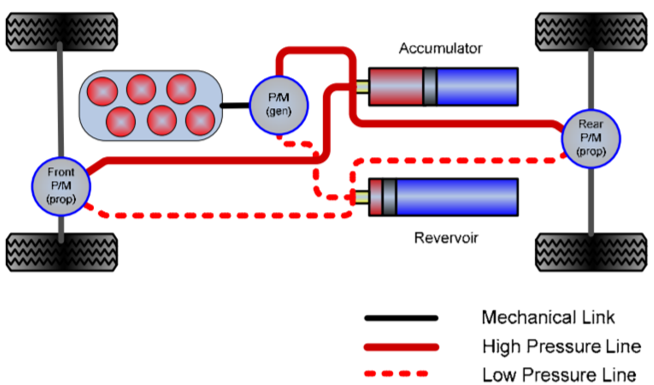
\includegraphics[width=.6\textwidth]{Images/Hydraulic KERS.png}
\caption{SHH scheme for a 4x4 vehicle}
\label{StepF1}
\end{figure}

The IC engine is mechanically coupled to the hydraulic pump/motor designated as P/M(gen). The P/M(gen) is used as a motor only when starting the engine. In all the other working conditions, the fluid pumped by P/M(gen) flows towards the P/M(prop-s) and the high pressure accumulator. Traction pumps/motors (P/Mprop-s) are connected to the wheels through a differential to provide propulsion. The pump/motor is a reversible energy conversion component. In particular, operating the P/M(prop) in the motor mode propels the vehicle, while regenerative braking requires switching to the pump mode. During the breaking phase, the hydro-pneumatic accumulator allows energy storage: as the P/M(prop), working as a pump, transfers the hydraulic fluid from the reservoir into the accumulator, the pressure of the gas sealed inside it increases, thus storing energy \cite{e}. In the accumulator (fig. 2), a bladder is used to separate the working fluid from the pressurized inert gas (e.g. nitrogen), which can be thus treated as a closed system. In a later acceleration event, the energy stored in the high pressure fluid contained in the accumulator is used, together with an amount delivered by the P/M(gen), to provide torque to the wheels. The pressure difference between the accumulator and the reservoir determines the maximum torque available from the hydraulic motor. In this phase, the working fluid is at least partially returned to the reservoir. 

\begin{figure}[H]
\centering
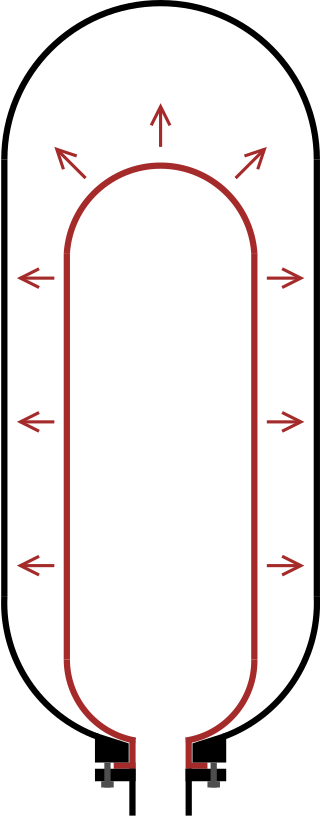
\includegraphics[width=.1\textwidth]{Images/Hydraulic Accumulator.png}
\caption{Bladder-type hydraulic accumulator}
\label{StepF1}
\end{figure}

The Reservoir is structurally similar to the accumulator but the gas that it contains is kept at low pressures and serves primarily to assist the transfer of fluid to-and-from the accumulator, with a minimal impact on the overall energy conversion. 

\subsubsection{Advantages, disadvantages and fields of application}

In contrast to its electric counterpart, fluid power technology is characterized by a higher power density and lower energy density \cite{f}. Energy density, which is also known as specific energy, represents the amount of energy that can be stored in a given mass of the system. On the other hand, energy density does not give information on how quickly this energy can be used: this knowledge is contained in the system's power density, which describes the rate at which its energy can be outputted. Moreover, since they release their energy more quickly, higher power density systems can also recharge more quickly. This feature makes hydraulic hybridization particularly interesting for applications with high and fast power transients.  In particular, utilization of hydraulic propulsion and energy storage components can offer significant advantages for those heavy vehicles that are required frequent start-stop operations, such as city buses, delivery vehicles and refuse trucks. It’s worth noticing that, in those fields of application, the stored energy is not necessarily limited to aid subsequent acceleration events, but can potentially represent a power source for the activation of ancillary equipment, as for example the compacting and packing mechanisms of refuse trucks. In addition, hydraulic KERS are also likely to have a longer operating life than battery-powered systems.  Another remarkable advantage of those systems is their high energy conversion efficiency: the state-of-the art bladder type accumulators with elastomeric foam can reach a round-trip efficiency of about 95\%. Once again, the combination of high efficiency and high charging-discharging rates enables particularly effective regeneration and re-use of hydraulic energy in heavy vehicles.
The main disadvantage of hydro-pneumatic KERS is represented by their high weight, which is mainly due to the presence of the working fluid and accumulators. This causes the specific energy of those systems to be relatively low. As a result, hydraulic hybrid systems encounter important limitations where consistent levels of power are required for extended periods at near constant speeds, such as in long-distance cruising.
Additional costs, which may represent 10–15\% of the total for the vehicle, is undoubtedly a further important drawback.

\subsection{Hydro-electric KERS}




%Codice per inserire le figure
\begin{comment}
\begin{figure}[H]
\centering
\includegraphics[width=.6\textwidth]{Charts/StepF1}
\caption{Step response of the closed--loop relative to $F_1$}
\label{StepF1}
\end{figure}
\end{comment}


%Codice per inserire il codice
\vspace{4cm}
This is a fancy in--line code
\singlespacing
\begin{Verbatim}[tabsize = 4, frame = lines, numbers = left]
code_here...
	code_here...
code_here...
\end{Verbatim}
\onehalfspacing


\begin{thebibliography}{3}
	
	\bibitem{a}
	J. Chibulka , “Kinetic Energy Recovery system by means of Flywheel Energy 		    storage device”. 
	Advanced Engineering, vol. 3, issue 1, pp. 27-38, 2009.
	
	\bibitem{b}
	R. Chicurel, “A Compromise Solution for Energy Recovery in Vehicle Braking”.      	Energy, vol.24, pp. 1029-1034, 2009.
	
	\bibitem{c}
	A. Harb. “Energy harvesting: State-of-the-art”. 
	Renewable energy, vol. 36, pp. 2641-2654, 2011.
	
	\bibitem{d}
	K. Baer et Al. “Robustness and performance evaluations for simulation-based 		control and component parameter optimization for a series hydraulic hybrid 			vehicle”,  Engineering Optimization 2020, VOL. 52, NO. 3, 446–464.	
	
	\bibitem{e}
	Y. J. Kim et Al., “Simulation Study of a Series Hydraulic Hybrid Propulsion 		System for a Light Truck”. SAE International, 2007.
	
	\bibitem{f}
	M. Shan “Modelling and Control Strategy for Series Hydraulic Hybrid 				Vehicles”.  PhD thesis, 2009.
	
\end{thebibliography}

\end{document}
